% Appendix (submitted as a separate supplementary PDF)
\appendix
\section{Rule Implementation Details}
\label{app:implementation}
This appendix shows how the Rule Generator implements a distilled rule as C++ code (Section~\ref{sec:offline:implement}).
We use \texttt{JoinDecomposeToPreagg\-regatedCount}, the highest-priority rule distilled from Stats-CEB query~88, as our running example.

\textbf{Prompt:}
Figure~\ref{fig:prompt} shows the prompt that the Rule Generator sends to the LLM.
It has seven parts.
Part~1 sets the role of the LLM as a C++17 developer for the rule engine.
Part~2 gives the \texttt{Rule} API, including the \texttt{Matches()} and \texttt{Apply()} signatures and the accessors of each operator type.
Parts~3 to~5 give the formal rule: the applicability condition $\phi_{r^*}$, the transformation $\tau_{r^*}$, and the fragment keys $\mathcal{K}_{r^*}$.
Part~6 provides the source-and-rewritten query pair $(Q, Q'')$ from which the rule was distilled.
Part~7 states the task and a strict output format: compilable C++17 code for the two methods, with no explanation and no markdown.
This structure grounds the LLM in the engine API and in one concrete example, and it keeps the output ready for compilation.

\begin{figure}[b!]
    \centering \vspace{0.35cm}
    \resizebox{.99\columnwidth}{!}{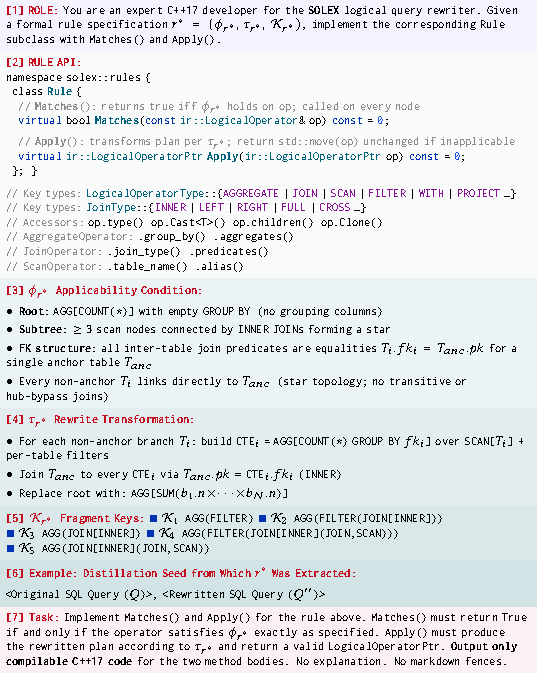
\includegraphics[scale=1]{figures/img/fig_Prompt}}
    \vspace{-0.15cm}
    \caption{LLM prompt for implementing the rule \texttt{JoinDecomposeToPreaggregatedCount}.}
    \label{fig:prompt}
    %\vspace{-0.5cm}
\end{figure}

\textbf{Generated Code:}
Figure~\ref{fig:code_example} shows the class that the LLM generates from the prompt above.
\texttt{Matches()} (Figure~\ref{fig_match}) returns true for a global \texttt{COUNT(*)} with no \texttt{GROUP BY} over a star join of at least three tables.
It checks that every join predicate is an equality between a branch table and one anchor table, and that each branch links directly to the anchor.
\texttt{Apply()} (Figure~\ref{fig_apply}) builds one CTE per branch that counts its rows per join key, with the branch filters pushed into the CTE.
It joins the anchor with these CTEs and replaces the root \texttt{COUNT(*)} with the sum of the products of the branch counts.
So one large join is replaced by one pre-aggregation per branch.
Neither method relies on table names, column names, or constants, so the same class handles any number of branches and concrete tables.
The class is compiled and loaded into the engine through \texttt{dlopen}~\cite{dlopen}, and then verified as described in Section~\ref{sec:offline:verify}.

\begin{figure}[b!]
    \centering %\vspace{-0.15cm}
    \resizebox{.99\columnwidth}{!}{
      \subfigure[\label{fig_match}\texttt{Matches()}: a global \texttt{COUNT(*)} over an $N$-table star join.]{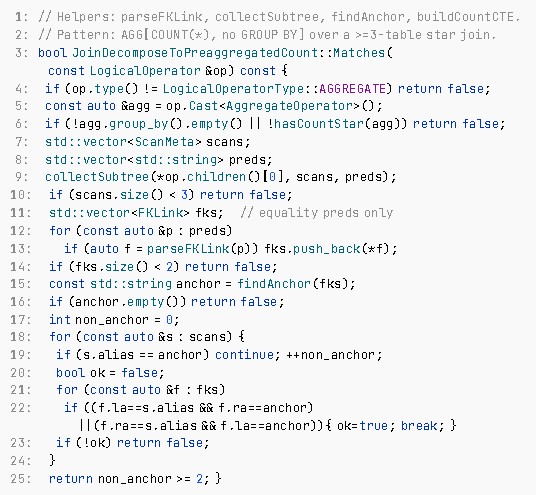
\includegraphics[scale=0.99]{figures/img/fig_CodeExampleMatch}}}

    \resizebox{.99\columnwidth}{!}{\subfigure[\label{fig_apply}\texttt{Apply()}: rewrite into pre-aggregated CTEs.]{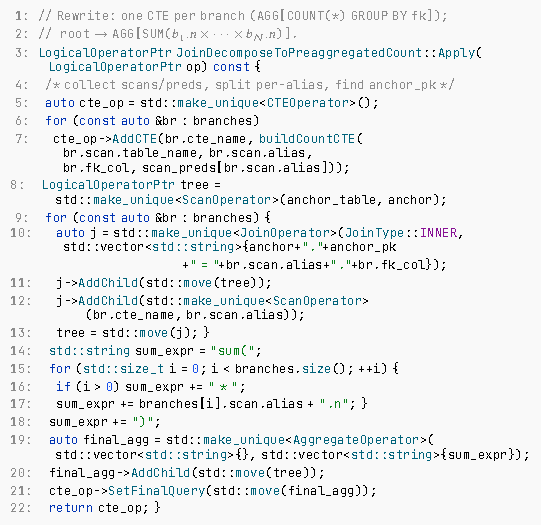
\includegraphics[scale=0.99]{figures/img/fig_CodeExampleApply}}}
    \vspace{-0.5cm}
    \caption{Generated C++ implementation of the rule \texttt{JoinDecomposeToPreaggregatedCount}.}
    \label{fig:code_example}
    %\vspace{-0.35cm}
\end{figure}

\newpage
\section{Rule Verdicts}
\label{app:rule_verdicts}
\blue{Table~\ref{tbl:rule_verdicts} breaks the rule verdicts of Section~\ref{sec:exp:verification} down by workload. For each workload, it reports the number of rules generated from its sampled queries, the number of rules of the pooled library that fire on its queries in at least one of the three dialects, and how many of these rules SQLSolver proves on at least one rewritten query or leaves undecided. The last row counts distinct rules, since a rule can be generated from, and fire on, several workloads.}

\begin{table}[H]
    \centering
    \caption{\blue{Rule Verdicts per Workload, Over All Three Dialects: Rules Generated From the Workload (Table~\ref{tbl:datasets}), Rules of the Pooled Library That Fire on It, Rules With at Least One Rewrite Proven by SQLSolver, and Rules SQLSolver Leaves Undecided.}}
    \label{tbl:rule_verdicts}
    \resizebox{0.99\columnwidth}{!}{
        \small \setlength\tabcolsep{3pt}
        \begin{tabular}{lrrrr}
        \toprule
        \textbf{Workload (\# Queries)} & \textbf{Generated} & \textbf{Fired} & \textbf{Proven} & \textbf{Undecided} \\ \midrule
        TPC-H (22)                   & 12 & 11  & 6   & 5  \\
        DSB (53)                     & 25 & 15  & 6   & 9  \\
        Stats-CEB (146)              & 16 & 15  & 10  & 5  \\
        Stats (146)                  & -- & 15  & 10  & 5  \\        
        JOB (113)                    & 19 & 18  & 10  & 8  \\
        JOB-Complex (30)             & 18 & 17  & 4   & 13 \\
        IMDB Full (13,646)           & 23 & 23  & 0   & 14 \\
        CEB (16)                     & -- & 14  & 0   & 14 \\
        StackOverflow (18,251)       & 12 & 12  & 7   & 5 \\
        StackOverflow SF\,1 (1,190)  & -- & 12  & 7   & 5  \\
        StackOverflow SF\,12 (1,190) & -- & 12  & 7   & 5  \\        
        \midrule
        Total (distinct rules)       & 67 & 67 & 37 & 30 \\
        \bottomrule
        \end{tabular}
    }
\end{table}
